\section{Affine $n$-Space and Algebraic Sets}\label{section_1.2}

\begin{definition}
  Let $k$ be a field. We define \textbf{affine $n$-space} over $k$ to
  be the cartesian product
  \begin{equation*}
    \A^n(k)=\underbrace{k \times \dots \times k}_{n\text{--times}}
    = k^n
  \end{equation*}
  We call the elements of $\A^n(k)$ \textbf{affine points} (or simply
  \textbf{points}). We call $\A^1(k)$ the \textbf{affine line} over
  $k$, and $\A^2(k)$ the \textbf{affine plane} over $k$. When the
  field $k$ is understood, we may simply write $\A^n$.
\end{definition}

\begin{definition}
  Let $k$ be a field, and let $f(x_1, \dots, x_n) \in k[x_1, \dots,
  x_n]$. We call an affine point $P \in \A^n(k)$ a \textbf{root}, or a
  \textbf{zero} of $f(x_1, \dots, x_n)$ if $f(P)=0$; where
  $f(P)=f(a_1, \dots, a_n)$ whenever $P=(a_1, \dots, a_n)$. We define
  the \textbf{zero-locus} (or \textbf{locus}) of $f(x_1, \dots, x_n)$
  to be:
  \begin{equation*}
    V(f)=\{P \in \A^n(k) : f(P)=0\}
  \end{equation*}
  If $S \subseteq k[x_1, \dots, x_n]$ is any set of polynomials, then
  the \textbf{zero-locus} of $S$ is defined to be:
  \begin{equation*}
    V(S)=\{ P \in \A^n(k) : f(P)=0 \text{ for all } f \in S \}
  \end{equation*}
  and if $S=\{f_1, \dots, f_r\}$, we write $V(S)=V(f_1, \dots, f_r)$.
\end{definition}

\begin{proposition}\label{proposition_10.1.1}
  Let $k$ be a field, and let $S \subseteq k[x_1, \dots, x_n]$ be any
  set of polynomials over $k$. Then:
  \begin{equation*}
    V(S)=\bigcap_{f \in S}{V(f)}
  \end{equation*}
  moreover if $S$ is finite, then $V(S)$ is a finite intersection.
\end{proposition}
\begin{proof}
  By definition, if $P \in V(S)$ then for any $f \in S$, $f(P)=0$ so
  that $P \in \bigcap{V(S)}$. Conversley if $P \in \bigcap{V(f)}$,
  then $f(P)=0$ for all $f \in S$, so $P \in V(S)$.
\end{proof}

\begin{definition}
  Let $k$ be a field. We call a subset  $X \subseteq \A^n(k)$ an
  \textbf{affine algebraic set} (or just \textbf{algebraic set}) if
  $X=V(S)$ for some set of polynomials $S \subseteq k[x_1, \dots,
  x_n]$.
\end{definition}

\begin{proposition}\label{proposition_10.1.2}
  Let $k$ be a field. Then the following statements about affine
  algebraic sets are true:
  \begin{enumerate}
    \item[(1)] If $\af \subseteq k[x_1, \dots, x_n]$ is an ideal
      generated by some set $S$ of polynomials over $k$ then
      $V(\af)=V(S)$.

    \item[(2)] If $\{\af_\a\}$ is some non-empty colleection of ideals
      in $k[x_1, \dots, x_n]$, then:
      \begin{equation*}
        V\Big{(} \bigcup_{\a}{\af_\a} \Big{)}=\bigcap_{\a}{V(\af_\a)}
      \end{equation*}

    \item[(3)] If $\af \subseteq \bf$, then $V(\bf) \subseteq V(\af)$.

    \item[(4)] Let $f,g \in k[x_1, \dots, x_n]$. Then $V(fg)=V(f) \cup
      V(g)$. Moreover, if $\af, \bf $ are ideals, in $k[x_1, \dots,
      x_n]$, then:
      \begin{equation*}
        V(\af\bf)=V(\af) \cup V(\bf)
      \end{equation*}
      Indeed, finite unions of algebraic sets are algebraic.

    \item[(5)] $V(0)=\A^n(k)$ and $V(1)=\emptyset$. Moreover,
      $V(x_1-a_1, \dots, x_n-a_n)=\{(a_1, \dots, a_n)\}$ for any $a_1,
      \dots, a_n \in k$.
  \end{enumerate}
\end{proposition}
\begin{proof}
  \begin{enumerate}
    \item[(1)] Let $\af=(S)$, and let $P \in V(\af)$. Then by
      definition, since $S \subseteq \af$, for any $f \in S$ $f(P)=0$
      so that $P \in \bigcap{V(f)}=V(S)$. So $V(\af) \subseteq V(S)$.
      On the other-hand, let $f \in \af$ and $P \in V(S)$. Since $\af$
      is generated by $S$ there are $\{f_\a\} \subseteq S$ such that
      \begin{equation*}
        f(x_1, \dots, x_n)=\sum_{\a}{g_\a(x_1, \dots, x_n)f_\a(x_1,
        \dots, x_n)}
      \end{equation*}
      where $g_\a \in k[x_1, \dots, x_n]$. Then sine $f_\a(P)=0$ for
      all $\a$
      \begin{equation*}
        f(P)=\sum_{\a}{g_\a(P)f_\a(P)}=0
      \end{equation*}
      so $P \in V(\af)$ and $V(S) \subseteq V(\af)$.

    \item[(2)] Take $\af=\bigcup{\af_\a}$ for some index $\a$. Let $P
      \in V(\af)$, so for any $f \in \af$ $f(P)=0$. But $f \in \af_\a$
      for some $\a$, hence $P \in V(\af_\a)$ for any $\a$. This puts
      $P  \in \bigcap{V(\af_\a)}$. Conversely, if $P \in
      \bigcap{V(\af_\a)}$, then $P \in V(\af_\a)$ for all $\a$, so
      that $P \in V(\af)$.

    \item[(3)] Let $\af \subseteq \bf$ be ideals in $k[x_1, \dots,
      x_n]$. Take $P \in V(\bf)$. Then for every $f \in \bf$,
      $f(P)=0$, by hypothesis, this makes $g(P)=0$ for every $g \in
      \af$. So $P \in V(\af)$.

    \item[(4)] Let $f,g \in k[x_1, \dots, x_n]$. Take $P \in V(fg)$.
      Then $fg(P)=f(P)g(P)=0$. Since $k$ is an integral domain, either
      $f(P)=0$ or $g(P)=0$, so $P \in V(f)$ or $P \in V(g)$.

      Conversely suppose that $P  \in V(f) \cup V(g)$. Then either
      $f(P)=0$ or $g(P)=0$. In either case we get $f(P)g(P)=fg(P)=0$
      so $P \in V(fg)$.

      Now, let $\af, \bf \subseteq k[x_1, \dots, x_n]$ be ideals, and
      let $P \in V(\af) \cup V(\bf)$. Then for any $f \in \af$ or for
      any $g \in \bf$ either $f(P)=0$ or $g(P)=0$. This puts $P \in
      V(\af\bf)$. Indeed if $\{\af_i\}_{i=1}^r$ is a family of ideals,
      and $\af=\prod_{i=1}^r{\af}$, then it follows from the above
      arguments that:
      \begin{equation*}
        V(\af)=\bigcup_{i=1}^r{V(\af_i)}
      \end{equation*}

    \item[(5)] Observe first that $V(0) \subseteq \A^n(k)$. Now let $P
      \in \A^n(k)$ having coordinates $P=(a_1, \dots, a_n)$. Then
      \begin{equation*}
        0(P)=\sum{0a_1^{d_1} \dots a_n^{d_n}}=0
      \end{equation*}
      so that $P \in V(0)$. Likewise, let $P \in V(1)$. Then $1(P)=0$.
      But also notice that:
      \begin{equation*}
        1(P)=1+\sum{0a_1^{d_1} \dots a_n^{d_n}}=1
      \end{equation*}
      which makes $1=0$ in $k$, which is impossible. Hence
      $V(1)=\0$.

      Lastly, let $P=(a_1, \dots, a_n)$. Then $P \in V(x_1-a_1, \dots,
      x_n-a_n)$ since $a_i-a_i=0$ for any $x_i-a_i$. Now, let $P \in
      V(x_1-a_1, \dots, x_n-a_n)$. Then for any $f \in (x_1-a_1,
      \dots, x_n-a_n)$ we get, letting $P=(b_1, \dots, b_n)$
      \begin{equation*}
        f(P)=(b_1-a_1)g_1(P)+\dots+(b_n-a_n)g_n(P)=0
      \end{equation*}
      which makes $b_i=a_i$ for all $1 \leq i \leq n$. This
      establishes that $V(x_1-a_1, \dots, x_n-a_n)=\{(a_1, \dots,
      a_n)\}$.
  \end{enumerate}
\end{proof}

\begin{example}\label{example_10.1}
  \begin{enumerate}
    \item[(1)] The following curves in figure \ref{figure_1.1} define
      algebraic sets over $\R$.
      \begin{figure}[h]
        \centering
        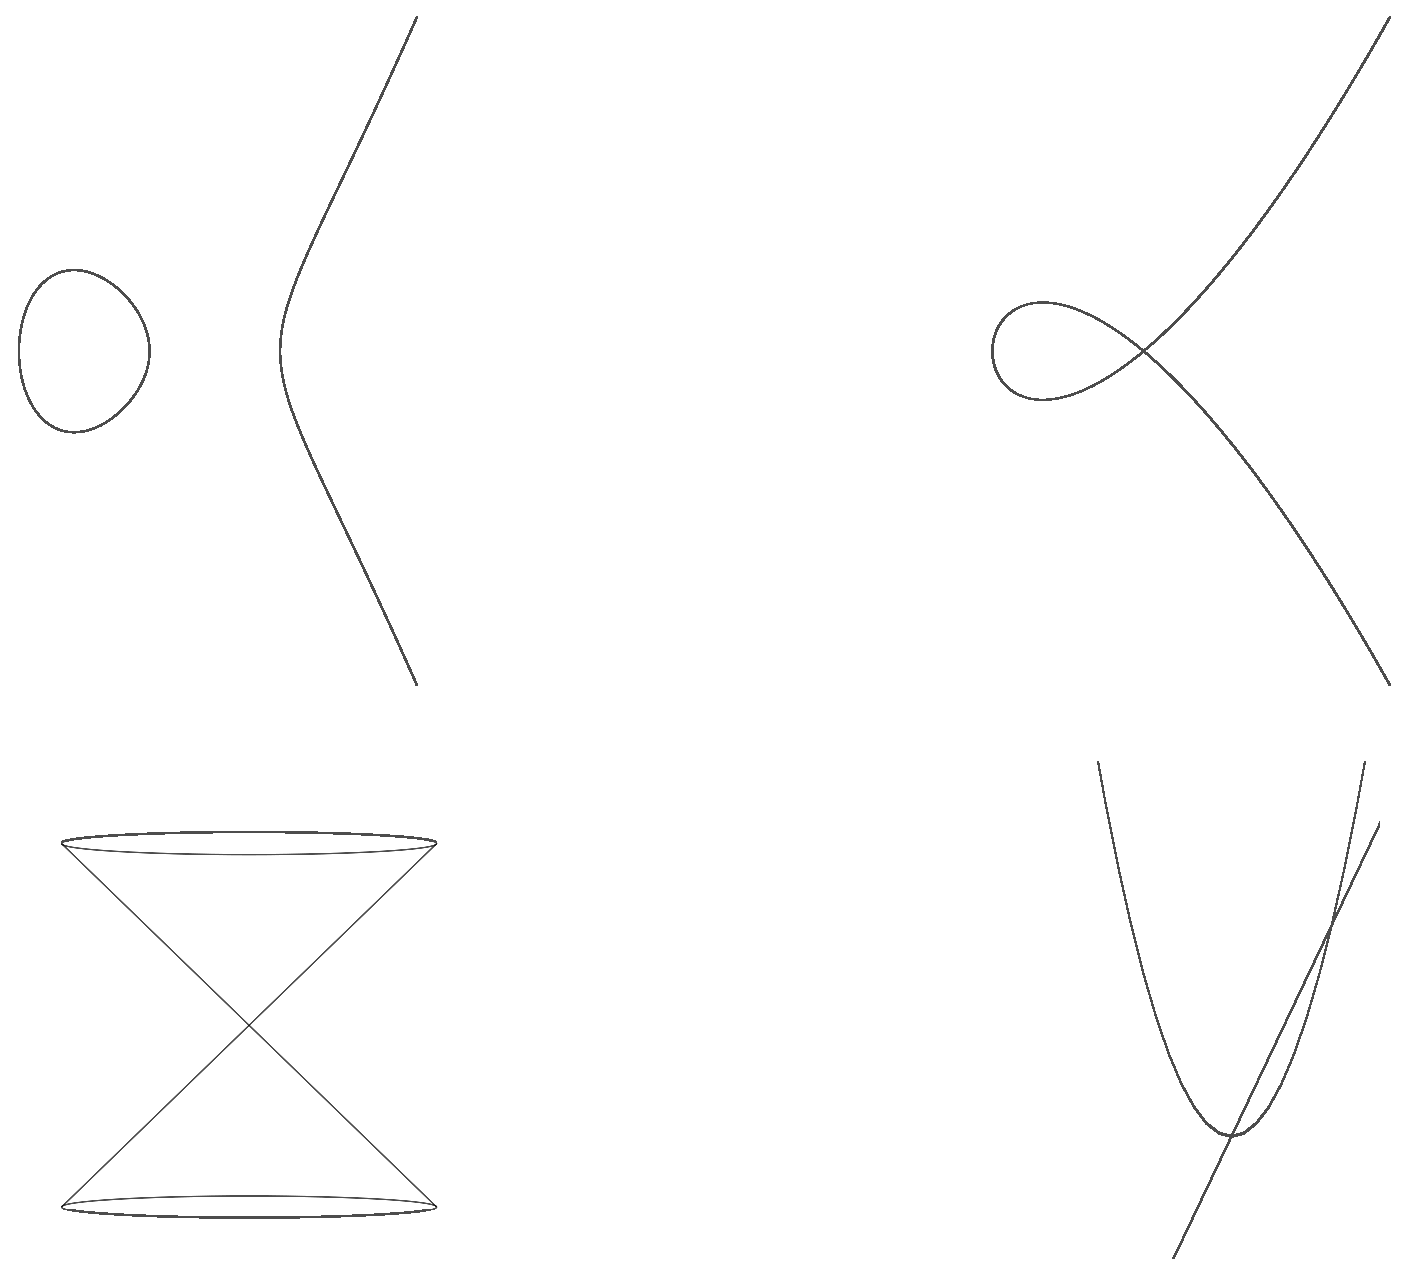
\includegraphics[scale=0.5]{parts/algebraic_curves/figures/Chapter1/hyperplanes.eps}
        \caption{Affine Algebraic Sets in $\A^2(\R)$ and $\A^3(\R)$.}
        \label{figure_1.1}
      \end{figure}

    \item[(2)] Let $k$ be any field, and let $X \subseteq \A^1(k)$ be
      an algebraic set. Then $X=V(S)$ for some set $S \subseteq k[x]$
      of polynomials. However, observe that for any $f(x) \in S$, with
      $\deg{f}=n$ that $f(x)$ has at most $n$ roots in $k$. Then
      $|V(f)| \leq n$. Now, since
      \begin{equation*}
        V(S) = \bigcap_{f \in S}{V(S)}
      \end{equation*}
      $|X|=|V(S)|$ is finite in $\A^1(k)$. Now also observe that
      $\A^1(k)=V(0)$. So the algebraic sets of $\A^1(k)$ are those
      finite point-sets, and $\A^1(k)$ itself.

    \item[(2)] Let $k$ be any field, and let $X \subseteq \A^n(k)$ be
      a finite point-set. Then $X=\{P_1, \dots, P_r\}$. Now let
      $P_i=(a_{i1}, \dots, a_{in})$. We have $V(x_1-a_{i1}, \dots,
      x_n-a_{in})=\{P_i\}$ so:
      \begin{equation*}
        X=\bigcup_{i=1}^r{V(x_1-a_{i1}, \dots, x_1-a_{in})}
      \end{equation*}
      which is an algebraic set by proposition
      \ref{proposition_10.1.2}.

    \item[(3)] Consider the finite field $\F_q$. Then the affine space
      $\A^n(\F_q)$ has exactly $q^n$ points. Hence if $X \subseteq
      \A^n(\F_q)$, then $|X| \leq q^n$ which makes $X$ a finite
      point-set, and hence it must be algebraic. Therefore every
      subset of $\A^n(\F_q)$ is algebraic.

    \item[(4)] For any $n \in \Z^+$, define $f_n(x)=x-n$ in $\Q[x]$.
      Then $V(f_n)=\{a_n\}$ in $\A^1(\Q)$, and we get the collection
      $\{V(f_n)\}_{n \in \Z^+}$ of algerbaic sets. However, observe
      that
      \begin{equation*}
        \bigcap_{n \in \Z^+}{V(f_n)}=\Z^+
      \end{equation*}
      which is infinite in $\A^1(\Q)$, and hence cannot be algerbaic.
  \end{enumerate}
\end{example}

\begin{example}\label{example_10.2}
  The following sets are algebraic.
  \begin{enumerate}
    \item[(1)] Consider $X=\{(t, t^2, t^3) \in \A^3(k) : t \in k\}$.
      Take $f(x,y,z)=x^3-z$ and $g(x,y,z)=x^2-y$. Then
      $f(t,t^2,t^3)=t^3-t^3=0$ and $g(t,t^2,t^3)=t^2-t^2=0$ so
      $X \subseteq V(f,g)$. On the other-hand if $P \in V(f,g)$ with
      $P=(a_1, a_2)$, then $f(P)=a_1^3-a_3=0$ and $g(P)=a_1^2-a_2=0$, so
      $P=(a_1, a_1^2, a_1^3)$. Which makes $V(f,g) \subseteq X$. We call
      the algebraic set
      \begin{equation*}
        V(x^3-z,x^2-y)=\{(t,t^2,t^3) \in \A^3(k): t \in k\}
      \end{equation*}
      the \textbf{twisted cubic} on $k$.

    \item[(2)] Let $X=\{(\cos{t}, \sin{t}) \in \R^2 : t \in \R\}$.
      Take $f(x,y)=x^2+y^2-1$. Then if $f(x,y)=0$ we get $x^2+y^2=1$
      which defines the unit circle $S^1$ in $\R^2$. Indeed,
      $X=V(x^2+y^2-1)$.

    \item[(3)] Let $X$ be the set of all points in $\R^2$ whose polar
      coordinates of the form $(r,\th)$ satisfy $r=\sin{\th}$. Indeed,
      let $(x,y) \in X$. Then
      \begin{align*}
        x^2+y^2 &= r^2 \\
                &= r\sin{\th} \\
                &= y \\
      \end{align*}
      that is: if $(x,y) \in X$ then $x^2+y^2-y=0$. Indeed define
      $f(x,y)=x^2+y^2-y$ in $\R[x,y]$. Then $X=V(f)$.

    \item[(4)] Let $k$ be any field, and choose $a,b \in k$. Define
      $f(x,y)=y-(ax+b)$. Then if $f(x,y)=0$ then $y=ax+b$. Conversely,
      if $P=(a_1, a_2)$ such that $a_1=\inv{a}(a_2-b)$ then observe
      that $f(P)=a_2-(a(\inv{a}(a_2-b))+b)=a_2-a_2=0$, so that
      \begin{equation*}
        V(y-(ax+b))=\{(a_1,a_2) \in \A^2(k) : a_1=\inv{a}(a_2-b)\}
      \end{equation*}
      Indeed, we have characterized all points for which $y=ax+b$.
      When $k=\R$, then $V(y-(ax+b))$ characterizes a line.
  \end{enumerate}
\end{example}

\begin{definition}
  Let $k$ be a field. We call the zero-locus of a non-constant
  polynomial $f(x_1, \dots, x_n) \in k[x_1, \dots, x_n]$ the
  \textbf{hypersurface} defined by $f(x_1, \dots, x_n)$. A
  hypersurface of degree $1$ is call a \textbf{hyperplane}. We call a
  hypersurface in $\A^2(k)$ an (\textbf{affine}) \textbf{plane curve}
  and we call a hyperplane in $\A^2(k)$ a \textbf{line}.
\end{definition}

\begin{theorem}\label{theorem_10.1.3}
  Let $k$ be any field, and let $C \subseteq \A^2(k)$ be an affine
  plane curve defined by a polynomial of degree $n$. If
  $L \subseteq \A^2(k)$ is a line such that $L \not\subseteq C$ then
  $L$ intersects $C$ at no more than $n$ points.
\end{theorem}
\begin{proof}
  Observe that if $L \subseteq C$ then $L \cap C=C$ and $L$ intersects
  $C$ at every point of  $C$.
  Now, by definition, since $L$ is a line, $L=V(y-(ax+b))$ for some
  $a,b \in k$. Now, let
  \begin{equation*}
    g(x)=f(x,ax+b)
  \end{equation*}
  in $k[x]$. Let $P \in L \cap C$ with $P=(x,y)$. Then $f(x,y)=0$ and
  $y-(ax+b)=0$ so that $f(x,ax+b)=0$ which puts $P \in V(g)$.
  Conversley, let $x \in V(g)$, then $g(x)=f(x,ax+b)=0$. Take $y=ax+b$
  for some $a,b \in k$. Then that we get the point $P=(x,y) \in L \cap C$.
  This makes $L \cap C=V(g)$. Since $V(g) \subseteq \A^1(k)$ and
  $\deg{g}=n$ we have that $V(g)$ contains no more than $n$ points.
\end{proof}
\begin{corollary}
  If $k$ is an algebraically closed field, then $L$ intersects $C$ at
  exactly $n$ points.
\end{corollary}

\begin{example}
  \begin{enumerate}
    \item[(1)] Let $C=\{(x,y) \in \R^2 : y=\sin{x}\}$. Let $L$ be the
      line defined by $f(x,y)=y-\frac{1}{2}$. Then $L \not\subseteq
      C$, and $L$ intersects $C$ at infinitely many points. Hence $C$
      is not an algebraic set in $\R^2$.

    \item[(2)] Let $X=\{(z,w) \in \A^2(\C) : |z|^2+|w|^2=1\}$, and
      suppose there were an $f(z,w) \in \C[z,w]$ for which $X=V(f)$.
      Define $g(z) \in \C[z]$ by $g(z)=f(z,0)$. Then $g(z)$ has
      finitely many roots, and $V(g)$ is finite in $\A^1(\C)$. Now,
      observe the point $P=(Z,0)$ in $X$ where $|Z|^2=1$. Then
      $g(Z)=f(Z,0)=0$ so that $Z \in V(g)$. However, letting $Z=X+iY$,
      observe that $|Z|^2=X^2+Y^2$ so that if $Z \in V(g)$, then
      $X^2+Y^2=1$, and so $Z \in S^1 \subseteq \A^1(\C)$. There are
      infinitely many such $Z$ which contradicts the finiteness of
      $V(g)$. Therefore $X$ cannot be algerbaic.

    \item[(4)] Let $X=\{(z,w) \in \A^2(\C): |z|^2+|w|^2=1\}$ as
      before. Let $z=x+iy$ and $w=u+iv$, and define
      $f(x,y,u,v)=(x^2+y^2)+(u^2+v^2)-1$ in $\R[x,y,u,v]$. Then
      $X=V(f)$, which makes $X$ algebraic in $\A^4(\R)$. Comparing
      this example to the previous, observe that since $\R^2 \simeq
      \C$, then $\A^4(\R) \simeq \A^2(\C)$. Now, $X$ is algerbaic in
      $\A^4(\R)$ but not in $\A^2(\C)$. Hence the isomoprphism of the
      spaces is not sufficient to determine whether a given set is
      algerbaic in on or the other.

    \item[(5)] Let $C=\{(\cos{t}, \sin{t}, t) \in \R^3 : t \in \R\}$
      and suppose there is an $f(x,y,z) \in \R[x,y,z]$ for which
      $C=V(f)$. Define $g(x)=f(\cos{(x+2\pi)}, \sin{(x+2\pi), x+2\pi})$
      in $R[x]$. Then if $t \in V(g)$, we get  $g(t)=
      f(\cos{(t+2\pi)}, \sin{(t+2\pi)}, t+2\pi)=f(\cos{t}, \sin{t},
      t+2\pi)$ and $(\cos{t+2\pi}, \sin{t+2\pi}, t+2\pi) \in C$.
      However there are infinitely such $t$ for which
      $\cos{t+2\pi}=\cos{t}$ and $\sin{t+2\pi}=\sin{t}$, which
      contradicts that $V(g)$ must be finite in $\A^1(\R)$. Therefore,
      $C$ cannot be algebraic.

    \item[(6)] Let $k$ be an algerbaically closed field, and let $f(x)
      \in k[x]$ be a non-constant polynomial. Then $V(f)$ has finitely
      many points in $\A^1(k)$; in fact $|V(f)|=\deg{f}$. It follows
      that $\com{\A^1(k)}{V(f)}$ is infinite. This holds for any
      non-constant polynomial $f(x) \in k[x]$, since $k[x]$ is a PID.

      Now, let $f(x_1, \dots, x_n) \in k[x_1, \dots, x_n]$ for $n>1$.
      Then we get
      \begin{equation*}
        f(x_1, \dots, x_n)=\sum_{i=1}^d{f_ix_n^i} \text{ where }
        f_i \in k[x_1, \dots, x_{n-1}]
      \end{equation*}
      is a polynomial of degree $d$ in $k[x_1, \dots, x_{n-1}][x_n]$,
      and hence has at-most $d$ roots in $\A^1(k)$. This makes $V(f)$
      finite in $\A^1(k)$ so that $\com{\A^n(k)}{V(f)}$ is infinite.

    \item[(7)] Let $k$ be an algerbaically closed field, and let
      $f(x,y) \in k[x,y]$. Then
      \begin{equation*}
        f(x,y)=\sum_{i=1}^d{f_i(x)y^i}
      \end{equation*}
      where $f_i(x) \in k[x]$. Now, since $k$ is algebraically closed,
      it is infinite. Hence, fix some $a \in k$, then
      \begin{equation*}
        f(a,y)=\sum_{i=1}^d{f_i(a)y^i}
      \end{equation*}
      and $f(a,y) \in k[y]$ has exacly $d$ roots in $k$. However, this
      holds for infinitely many $a \in k$ so that $f(x,y)$ must have
      innfinitely many roots in $k$. Hence $V(f)$ must be infinite in
      $\A^2(k)$. Indeed, observe that for any $n>2$ and $f(x_1, \dots,
      x_n) \in k[x_1, \dots, x_n]$ that $V(f)$ is infinite in
      $\A^n(k)$. We get
      \begin{equation*}
        f(x_1, \dots, x_n)=\sum{f_ix^{d_1}y^{d_2}}
      \end{equation*}
      where $f_i \in k[x_1, \dots, x_{n-2}]$ and $x=x_{n-1}$. Fixing
      $P \in \A^{n-2}(k)$, we get $f(P,x,y) \in k[x,y]$ must have
      infinitely many roots, for infinitely many points $P$.

    \item[(8)] Let $S \subseteq k[x_1, \dots, x_n]$, and let $\af=(S)$
      the ideal generated by $S$. Then foor any $f \in S$ the ideal
      $(f) \subseteq \af$ so $V(\af) \subseteq V(f)$ and
      $\com{\A^n(k)}{V(f)}$ is infinite. But $\com{\A^n(k)}{V(f)}
      \subseteq \com{\A^n(k)}{V(\af)}$. Therefore, the complement of
      any algerbaic set in $\A^n(k)$ is infinite.
  \end{enumerate}
\end{example}

\begin{defintion}
  Let $k$ be a field, and $X \subseteq \A^m(k)$ and $Y \subseteq
  \A^n(k)$. We define the \textbf{cartesiona product} of
  $X$ and $Y$ to be the set $X \times Y \subseteq \A^{m+n}(k)$ by:
  \begin{equation*}
    X \times Y=\{(P,Q) : P \in \A^m(k) \text{ and } Q \in \A^n(k)\}
  \end{equation*}
\end{defintion}

\begin{proposition}\label{proposition_10.1.4}
  If $X \subseteq \A^m$ and $Y \subseteq \A^n$ are algerbaic sets,
  then the cartesian product $X \times Y$ is algebraic in $\A^{m+n}$.
\end{proposition}
\begin{proof}
  Let $S \subseteq k[x_1, \dots, x_m]$ and $T \subseteq k[y_1, \dots,
  y_n]$. Let $\af=(S)$ and $\bf=(T)$ the ideals generated by $S$
  and $T$ respectively, and take $X=V(\af)$ and $Y=V(\bf)$. Now
  $\af=(f_1, \dots, f_r)$ and $\bf=(g_1, \dots, g_s)$, So let
  $f(x_1, \dots, x_m)=p_1f_1+\dots+p_rf_r$ and
  $g(y_1, \dots, y_n)=q_1g_1+\dots+q_sg_s$, and define
  \begin{equation*}
    h(x,y)=p(x)f(x)+q(y)g(y)
  \end{equation*}
  where $x=(x_1, \dots, x_m)$ and $y=(y_1, \dots, y_n)$. Then let
  $\cf$ the ideal generated by all $h(x,y) \in k[x,y]$. Let $R \in X
  \times Y$. Then $R=(P,Q)$ where $P \in X$ and $Q \in Y$. Then for
  some $p \in k[x_1, \dots, x_m]$ and $q \in k[y_1, \dots, y_n]$:
  \begin{equation*}
    h(R)=p(P)f(P)+q(Q)g(Q)=0
  \end{equation*}
  since $X=V(\af)$ and $Y=V(\bf)$. This puts $X \times Y \subseteq
  V(\cf)$. Conversely, let $R \in V(\cf)$. Recall that $\cf=(h_1,
  \dots, h_t)$ since $k[x,y]$ is Noetherian. Let $R \in V(\cf)$ have
  the form $R=(P,Q)$. Then for any $h(x,y)$ we have
  \begin{equation*}
    h(R)=l_1(R)h_1(R)+\dots+l_t(R)h(R)=0
  \end{equation*}
  So that $h_i(R)=0$. But recall that
  \begin{equation*}
    h_i(x,y)=p_i(x)f_i(x)+q_i(y)g_i(y)
  \end{equation*}
  where $f_i(x_1, \dots, x_m)=p_{i1}f_{i1}+\dots+p_{im}f_{im}$ and
  $g_i=q_{i1}g_{i1}+\dots+q_{in}g_{in}$. Hence $h_i(R)=0$ for all $1
  \leq i \leq t$ so that $f_i(P)=0$ and $g_i(Q)=0$, which puts $P \in
  X$ and $Q \in Y$. That is: $V(\cf) \subseteq X \times Y$. This makes
  $X \times Y$ algebraic.
\end{proof}

\begin{theorem}\label{theorem_10.1.5}
  Any algebraic set is the intersection of a finite number of
  hypersurfaces.
\end{theorem}
\begin{proof}
  Let $k$ be the given field and let $S \subseteq k[x_1, \dots, x_n]$
  be any set of polynomials, and let $\af=(S)$ the ideal generated by
  $S$. Again, since $k[x_1, \dots, x_n]$ is Noetherian, $\af=(f_1,
  \dots, f_r)$ for some $f_1, \dots, f_r \in S$. Moreover, by
  proposition \label{proposition_10.1.2}, $V(S)=V(\af)$. It follows
  from proposition \label{proposition_10.1.1} that
  \begin{equation*}
    V(\af)=\bigcap_{i=1}^r{V(f_i)}
  \end{equation*}
\end{proof}
